\section{Introduction}
With the excess of career opportunities in our society, it has become increasingly difficult to choose the right career path. This is an example of  the paradox of choice where having more options causes individual to struggle when making decisions, due to fear of making the wrong decision. Further, this indecisiveness causes a gap in the job market, filling jobs with individuals who are not passionate about their work, causing decreased levels of productivity. Our mission, is to limit the range of choices for prospective professionals, giving them the opportunity to better understand career paths based on their work experience and the current education and job market. 

\section{Related Work}
As of late companies are searching for ways to attract and retain top talent in order to further business initiatives. In turn,  research in the field of talent acquisition, retention and mobility is gaining a substantial amount of traction. Two studies specifically \cite{li2017, kapur2016}, applied data mining strategies to model talent career paths and career outcomes based on education respectively. 

The research team in \cite{li2017} sought to model talent career paths by focusing on turnover and career progression. Their study is focused on a dataset containing anonymized employee career data. For each employee, there is temporal data reflective of start/end dates of the employee joining the company or holding a position at a given occupational level. Further, their research was supplemented by both static and dynamic information for each employee. They describe static information as unchanged data such as gender and age. On the other hand, dynamic information included numeric performance ratings and hierarchical report chains with respective time stamps. The use of such dynamic factors provided a qualitative look at what governs an employee leaving a company or being promoted within a company which was unique in comparison to the datasets we were able to gather for analysis. The researchers found that without the numeric performance rating attribute the model's performance would decrease substantially, meaning that this attribute is a viable metric for predicting career path and status within a company.  All in all, the team proposed "a novel survival analysis approach for modeling the career paths of employees, which is based on multitask learning with ranking constraint formulation."\cite{li2017} which significantly outperformed other multi-task learning and survival analysis methods. 

The research team from LinkedIn \cite{kapur2016} leveraged valuable proprietary data in order to rank universities based on industry performance of their graduates. The team created a system with two main ranking components: a company ranker and school ranker. The company ranker used LinkedIn member data to generate desirable companies for a given profession. The school ranker was then used to rank universities based on the number of graduates attaining a job at a desirable company for a given profession. Their company ranker is a graphical model, where companies represent the nodes of the graph and employee movement from company to company is represented by the edges of the graph. Finally, in order to generate the desirability score of each company, the team applied PageRank on the graph. Using this company ranker they could then begin to generate university rankings. The research proposed by this group provided a novel approach to understanding the importance universities play in attaining a job for a given profession. They were able to analyze career= trajectories of graduates and use that information to generate a ranking for a university as opposed to other metrics based on "reputational assessments". Ultimately, the team's work provided substantial insight for universities and students; adding to the resources provided by LinkedIn Higher Education while gaining media coverage from major publishers.

Within our analysis, we sought to accomplish the following: gain insight on the current job and education market, mine user data relevant to career trajectories(LinkedIn profiles and resumes), use mined data to predict potential career paths. All in all, our research culminates a variety of data sources and data mining approaches to help prospective professionals make confident decisions in the job industry. 
\section{Methodology}
\subsection{Data Acquisition}
Gathering data began with searching for openly available datasets relevant to our problem statement. In turn, we gathered data relevant to the current education and job market, leading company data and user data. 
\begin{enumerate}
	\item Job Market data
	\begin{enumerate}
		\item US Jobs on Monster.com \cite{kaggleMonsterJobs}
		\begin{enumerate}
			\item Includes job listings of various US based positions. Provides, title, description, location, sector and organization of each listing 
			\item Provided us with a means for analyzing how job descriptions play a role in predicting job industry through the use of text analysis and classification methods
			\item Allowed us to mine popular locations amongst job listings 
		\end{enumerate}
	\end{enumerate}

	\item Company Data
	\begin{enumerate}
		\item Fortune 500 Companies \cite{fortune500}
		\begin{enumerate}
			\item List of top companies ranked by revenue
			\item Provided a means for tiering companies 
		\end{enumerate}
		\item The Open Data 500 \cite{kaggleCompanies}
		\begin{enumerate}
			\item General company metadata including: size, category, location, business model attributes 
			\item Provided data to analyze industry, company size and location popularity
		\end{enumerate}
	\end{enumerate}
	\item Education Data
	\begin{enumerate}
	\item College Scorecard Data \cite{collegeScorecard}
		\begin{enumerate}
			\item Contains relevant statistics about US universities including: admission rates, unemployment rates, post graduation earnings and degree percentages.
			\item Provided data for modeling salary expectations based on university type
			\item Allowed us to analyze correlation of admission rates and unemployment rates.
		\end{enumerate}
	\item University and Degree Data \cite{kaggleCollege}
		\begin{enumerate}
			\item Included 3 datasets regarding US universities and degree programs
			\item Salary by degree: earnings statistics for various degree programs 
			\item Salary by college type: earnings statistics for universities of a given type (Public, Ivy League, Party, Liberal Arts)
			\item Salary by region: earnings statistics for universities within given regions. (This dataset was joined with the college type dataset as they both contained the same universities.)
		\end{enumerate}
	\item The Times Higher Education World University Ranking 2018 \cite{timesHigher}
		\begin{enumerate}
			\item List of World Universities ranked
			\item Allowed for a means of tiering universities for predictive analysis
		\end{enumerate}
	\end{enumerate}
	\item User Data
	\begin{enumerate}
	\item Linkedin.com Scrapper \cite{linkedin}
		\begin{enumerate}
			\item Extraced previous work and education experience
			\item Used to model career paths
		\end{enumerate}
	\item Indeed.com Scrapper \cite{indeed}
		\begin{enumerate}
			\item Extracted job title, education and 3 most recent work experiences based on job query 
			\item Collected a total of records to use in conjunction with linkedin data to predict (add more)
		\end{enumerate}
	\end{enumerate}
\end{enumerate}

\subsection{File Structure}
\begin{forest}
	for tree={
		folder,
		grow'=0,
		align=left,
		child anchor=mid west,
	},
	[root
		[analysis 
			[college-scorecard-analysis.ipynb
				[code for analyzing College Scorecard Dataset \cite{collegeScorecard}]
			]
			[education-analysis.ipynb
				[code for analyzing Wall Street Journal University datasets \cite{kaggleCollege}]
			]
			[job-market-analysis-refined.ipynb
				[code for analyzing job listings from Monster.com dataset \cite{kaggleMonsterJobs}]
			]
			[trajectory-analysis-rev-ntr.py]
			[trajectory-analysis.py]
			[us-companies-analysis.ipynb
			]
		]
		[data
			[images: analysis generated images]
			[companies: company data \cite{fortune500, kaggleCompanies}]
			[education: data for education analysis \cite{timesHigher}]
			[jobs: job analysis data \cite{kaggleMonsterJobs}]
			[users: scraped user data \cite{linkedin, indeed}]
			[scraping: various scrapers]
		]
		[submission: all files related to PDF generation]
	]
\end{forest}

\section{Experiment}
\subsection{Job Listing Analysis}
To begin analysis of the job listing data we first sought to gain an understanding of the dataset by constructing visualizations of the data. Throughout this process we were able to gain insight into popular job locations, distribution of organization and sector values, and frequently occurring words within job titles.  As seen in Figure \ref{fig:test1}, healthcare and retail listings dominate this dataset which validates the important words found in the job title field due to the fact that "manager", "sales", "specialist", "technician" , "supervisor" are among the top ten most frequently occuring words. \\
\begin{figure} 
	  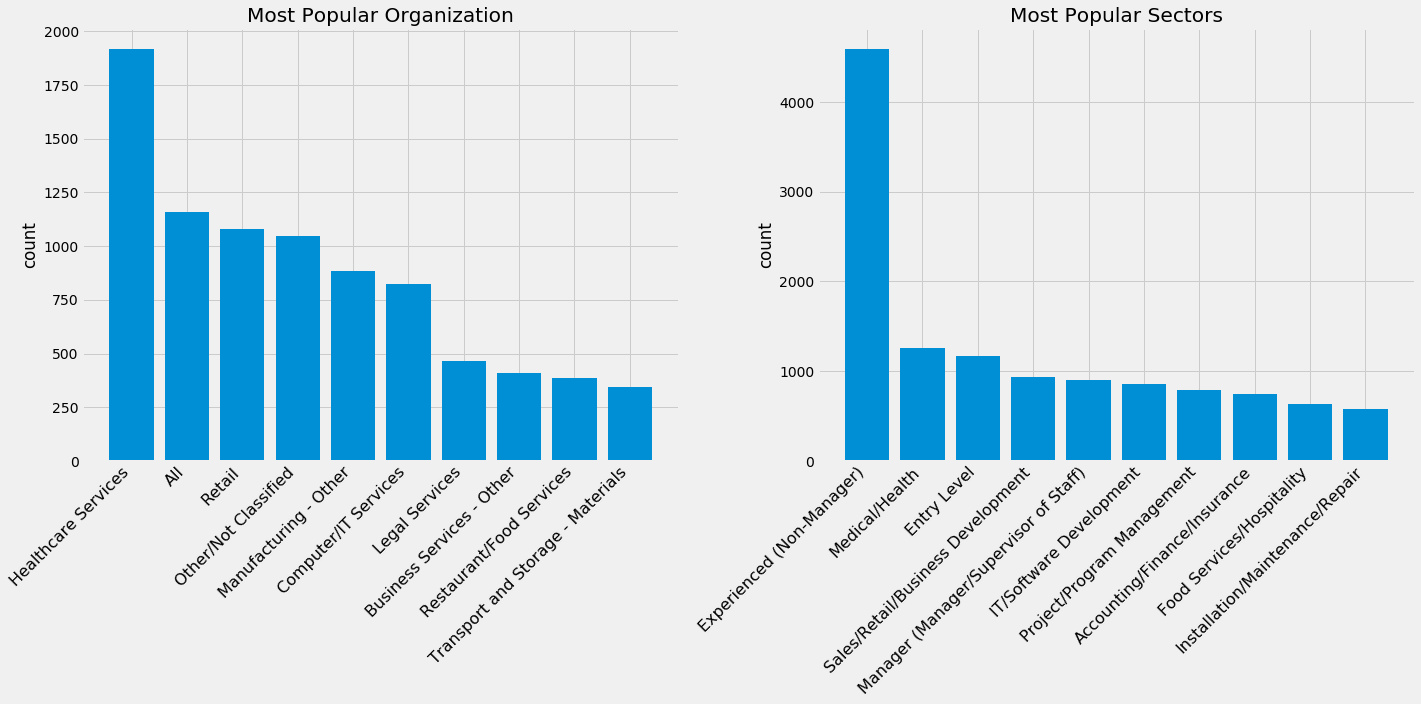
\includegraphics[width=\textwidth]{images/listings_freq.png}
	\captionof{figure}{}
	\label{fig:test1}
\end{figure}
\begin{figure} 
	  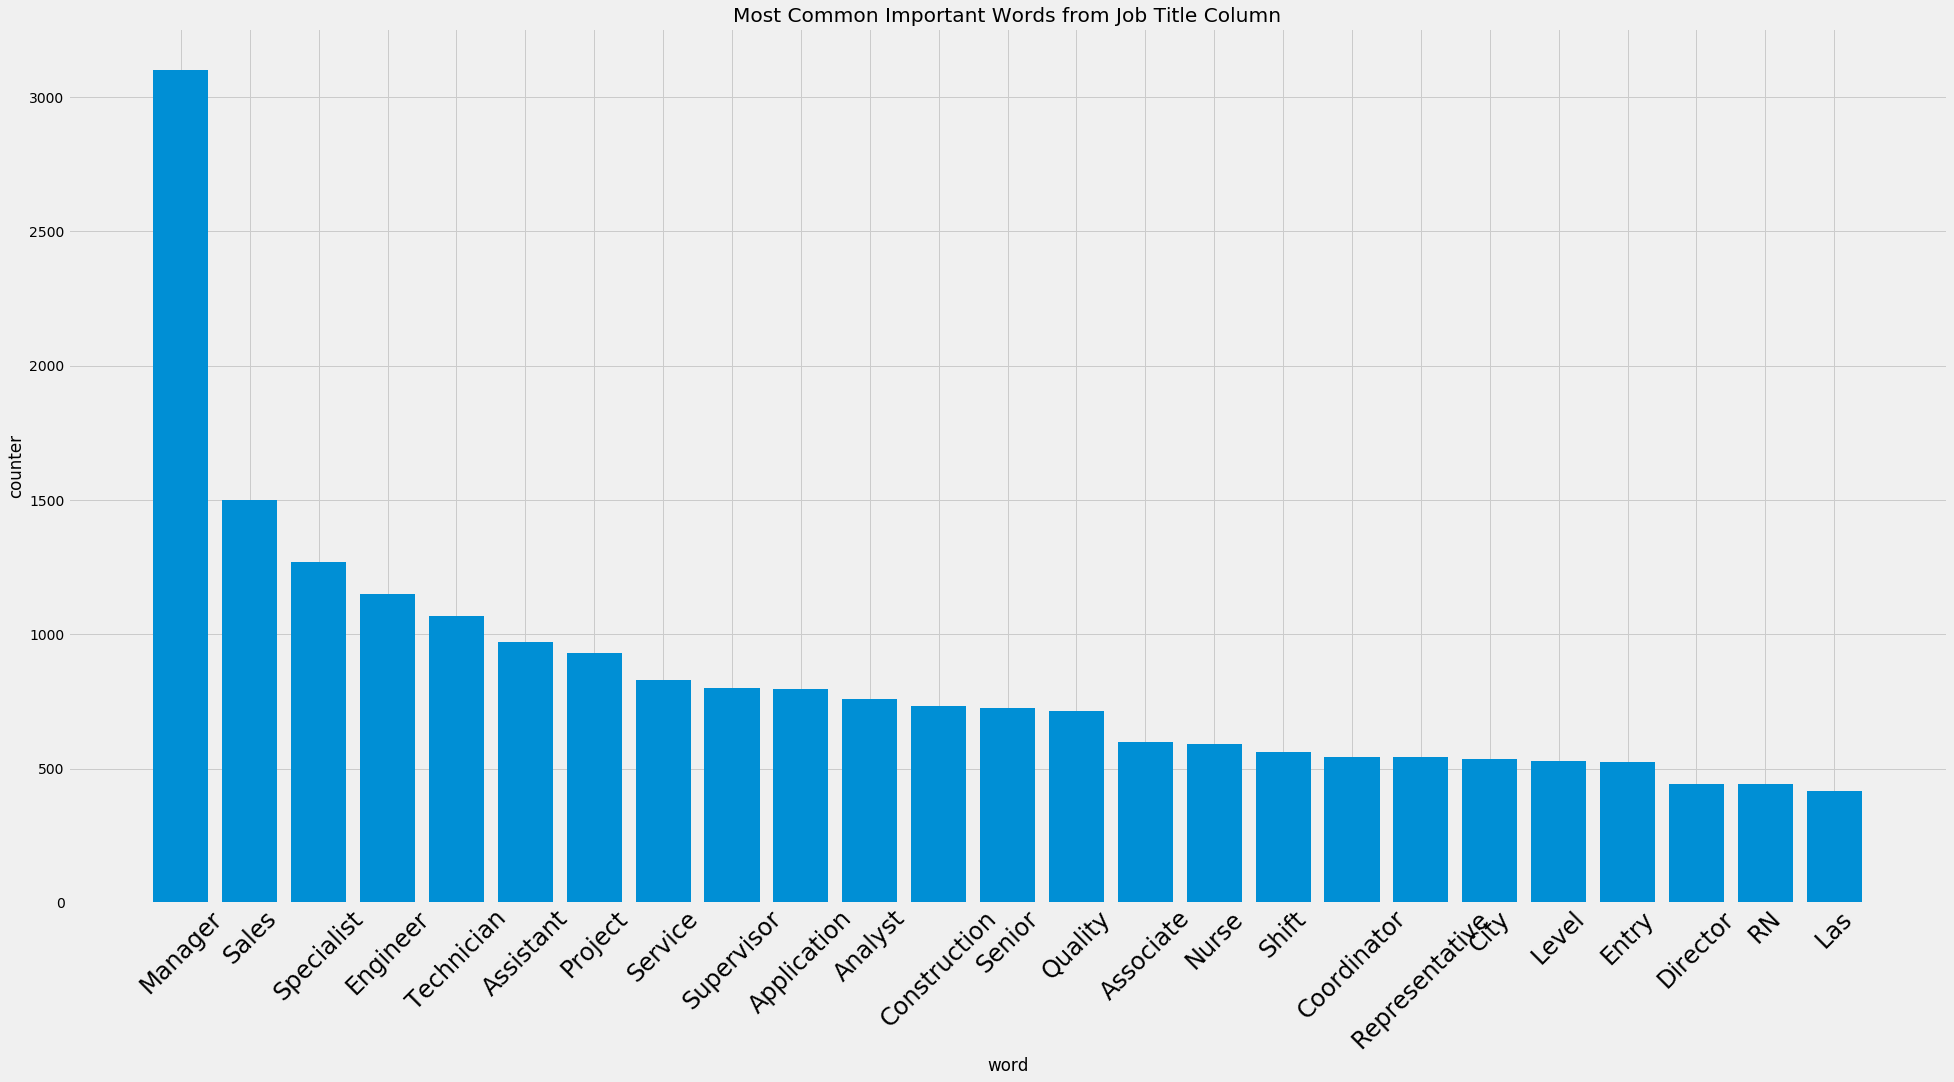
\includegraphics[width=\textwidth]{images/listing_title.png}
	\captionof{figure}{}
	\label{fig:test2}
\end{figure}



Next, we sought to analyze the job description field to see if we could use this attribute to determine what organization the listing corresponded to. The motivation here was that each organization would have a unique set of words within the description field that are exclusive to that organization and using this assumption we can create a consistent feature set for each job listing to train a classifier with. The following steps were taken in our text classification process:
\begin{enumerate}
	\item Feature Creation
	\begin{enumerate}
		\item Create of the bag-of-words 
		\begin{enumerate}
			\item Iterated through all job listings
			\item Removed irrelevant words(stop words) and punctuation
			\item Lemmatized each non-stop word in order to reduce derived words down to one common lemma. i.e.(walked, walks, walking = walk)
			\item Our bag-of-words contains the 1000 most frequent words 
		\end{enumerate}
			\item Use our bag-of-words to create a consistent feature set for each listing's description field
		\begin{enumerate}
			\item Given our bag-of-words of length 1000 we create a length 1000 feature vector
			\item Each index i in the feature vector corresponds to a binary value(1 if word is in description else 0) based on whether or not the word in index i of our bag-of-words is in the description of the current listing
		\end{enumerate}
	\end{enumerate}
	\item Label Creation
	\begin{enumerate}
		\item One hot encode organization values
		\item Given 5 organization values create a label vector of length 5 
		\item Each index of the label vector corresponds to a unique organization value 
		\item For each listing, set the listing's organization value index to 1 in the label vector, every other index will remain 0
	\end{enumerate}
\end{enumerate}

\subsection{Classification Process and Results}
After creation of our feature and label sets we were prepared for classification. The algorithms we used for classification were Naive Bayes and a Multilayer Neural Network. Our training and testing sets where split 75\%/25 (total = 6091 , training = 4568 , test = 1523) and the top 5 most common organization values were used as labels.  

\subsubsection{Naive Bayes}
We used two forms of Naive Bayes namely, Multinomial and Bernoulli Bayes. The core difference between these two algorithms is that Bernoulli Bayes can only operate with binary feature values but Multinomial Bayes can operate with both binary and absolute count feature values. The accuracy of our Naive Bayes classifiers were just over chance, attaining 64\% accuracy for Multinomial Bayes and 63\% for Bernoulli Bayes. 

\subsubsection{Multilayer Neural Network}
Our Multilayer Neural Network was designed using TensorFlow\cite{tensorFlow}. In order to create a neural network using TensorFlow, we had to create a computation graph to represent our neural network model which would then be run by a TensorFlow session with our input data. In order to create the computation graph, each layer's weights and biases were defined, then the computation between each layer was defined. The computation between each layer is simply (input data * weights) + biases applied to an activation function (reLu for classification purposes) where each layer is then passed as input data to the next layer. Next, we defined an optimization function to reduce the cost after each iteration of training. Finally, to ensure our network was operating appropriately, we ran our TensorFlow session in batches, outputting the loss to ensure that as the network was training the loss was decreasing. Ultimately, our neural network model attained an accuracy of 75\%.

\subsubsection{Job Listing analysis results}
Ultimately, organization prediction based on job description could be improved with a larger data set and cleaner data. The data set proved to be very sparse leaving us with a small fraction of the dataset to analyze(only 6091 listings out of 22,000). Therefore, given more data from a variety of job listings our text based classification approach could yield promising results.

\subsection{Education Analysis}
\subsubsection{College Scorecard data}
The motivation for analyzing the college scorecard data \cite{collegeScorecard} was to understand how various university metrics play a role in determining employment and earnings of prospective graduates. The main attributes of focus were admission rates, unemployment rates, and degree percentages(percentage of students awarded a given degree) for each university. One of the first metrics we analyzed was the correlation between admission and unemployment rates. Looking at the scatterplot below, it is evident that there is no correlation between admission and unemployment rates. This is an interesting finding because this contrary to the popular belief that universities with lower admission rates yield increased job placement. But after careful consideration, this lack of correlation can possibly be explained by universities with higher admission rates offering degree programs where the job market is less competitive and there are more readily available jobs. As opposed to universities with lower admission rates placing students in highly competitive fields. Another possible explanation could be that universities with lower admission rates are on average smaller than universities with higher admission rates. For example, two universities(one large, one small) with the same number of unemployed graduates, will lead to the smaller university having a higher unemployment rate than the larger university.
\begin{figure} 
	  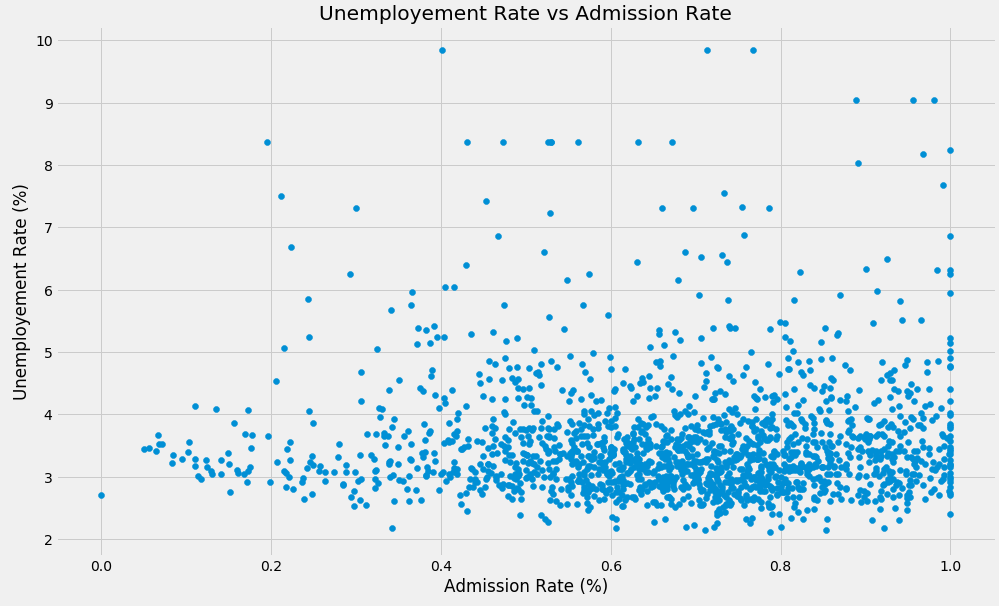
\includegraphics[width=\textwidth]{images/adm_unem_rate_scatter.png}
	\captionof{figure}{}
	\label{fig:test3}
\end{figure}


To further investigate the effects of university statistics on career outcomes we created a multivariate linear regression model.
In doing so, we used degree percentages, admission rates and unemployment rates as independent variables and median 10 year salary as our dependent variable.
The accuracy of the regression model is characterized by a standard error of ~25\% and $R^2$ value of .5. This tells us that the dependent variables play a moderately strong role in determining the salary of a graduate of a given university with relatively high accuracy. However, we noticed a potential source of bias within the data. We recognized that degrees for health professions were the most common degree type awarded, nearly doubling the next highest category. This imbalance could potentially skew our regression to favor salaries of health professions as opposed to the other degree programs. Therefore, we pruned universities which had health profession degree percentage attribute larger than 50\%. This yielded a .3 increase in our $R^2$ value and a ~5\% increase in accuracy.

Taking an even granular look at degree programs we were able to visualize percent change from start to mid career for various degree programs (Figure \ref{fig:test4}). The two lowest percent changes in salary were for Nursing and Physician Assistant degree programs. Our hypothesis for this finding is that these two degree programs do not adopt the typical corporate hierarchy. In order for nurses or physician assistants to advance to higher levels of the medical hierarchy, more schooling would be required. Overall, this is quite common in the medical field, in order for employees to advance more certification is inevitable. On the other hand, the majority of degree programs under study do adopt a corporate hierarchy where it is common for an employee to  "climb the corporate ladder". For example, a business student moving from an analyst, to an associate, to vice president, etc. Ultimately, the corporate hierarchy trend causes the mean percent change to be ~70\% while Nursing and Physician Assistant percentages are substantially lower ~50\%. 
\begin{figure} 
	  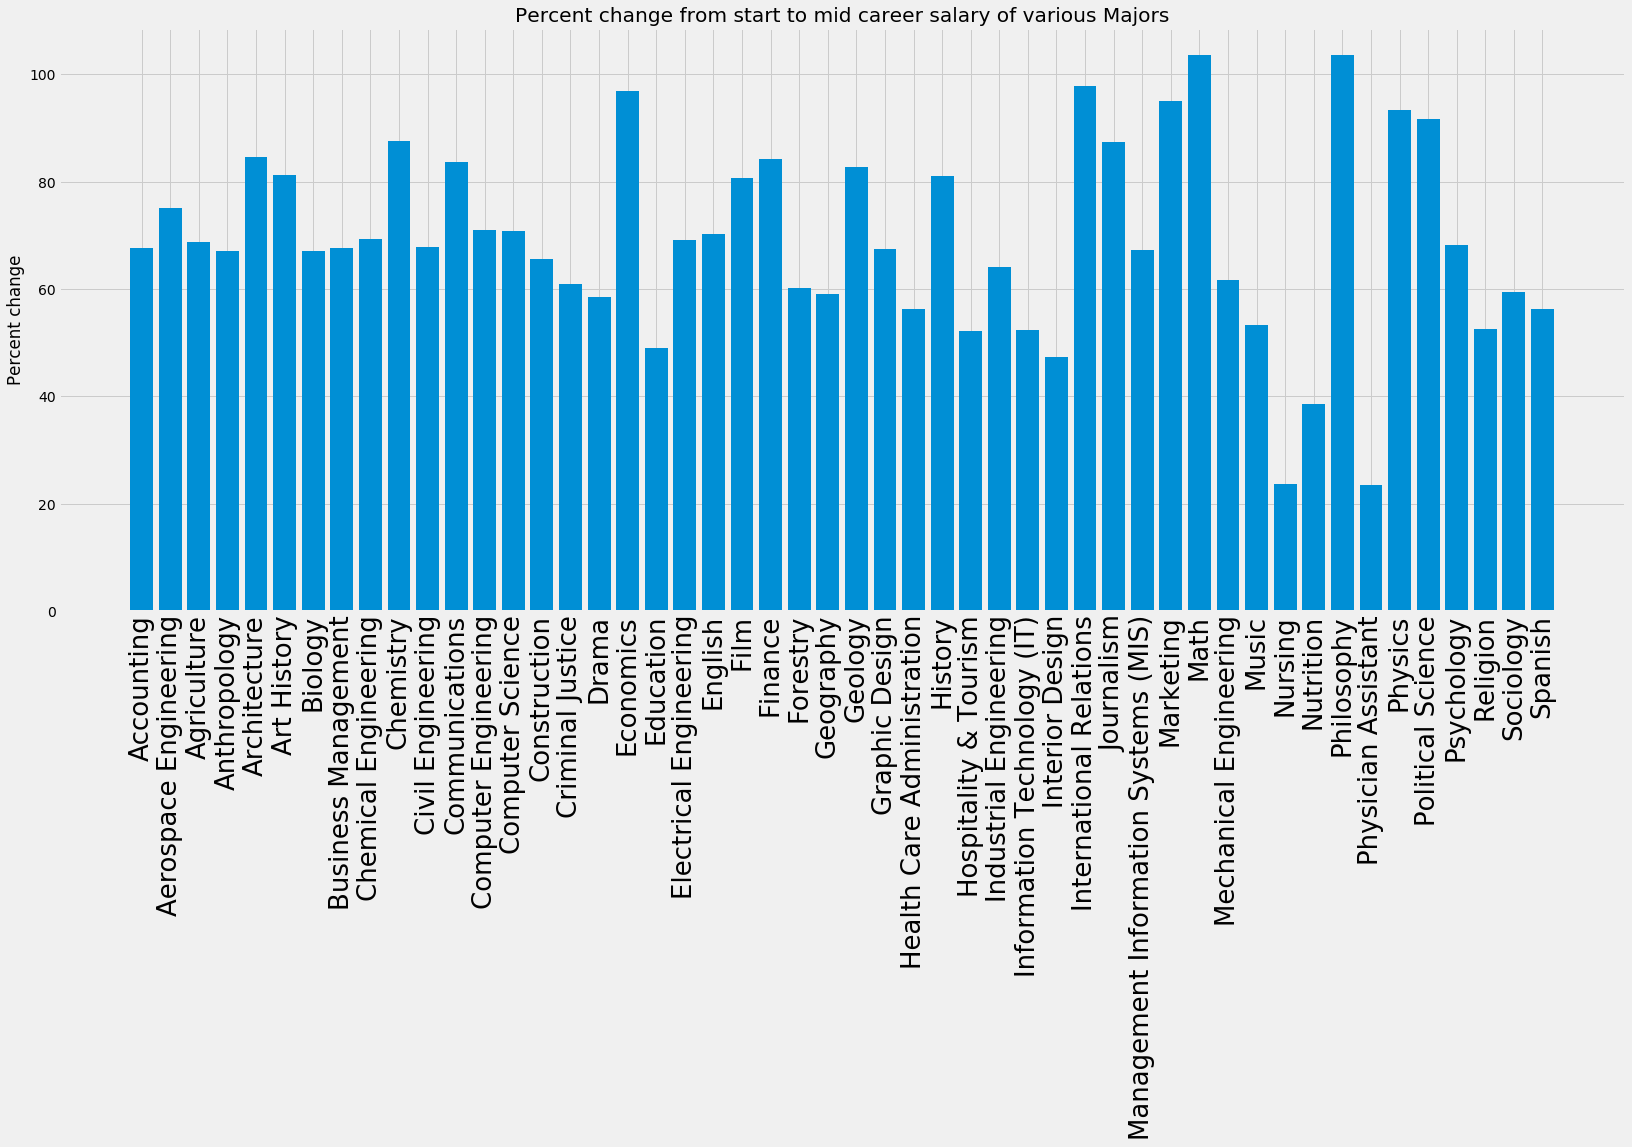
\includegraphics[width=\textwidth]{images/major_pct_chg.png}
	\captionof{figure}{}
	\label{fig:test4}
\end{figure}


\subsection{Company Analysis}
To further supplement our predictive modelling of career outcomes we sought to extract various characteristics of industry leading companies. For example, when analyzing the The Open Data 500 dataset \cite{kaggleCompanies}, we found that the most popular company categories were data/technology and Finance/Investment validating the high frequency of company locations being in Silicon Valley and New York. Further, startups dominate this data set, Figure \ref{fig:test6} shows over 50\% of companies having less than 50 employees. \\
\begin{figure}
	\centering
	\begin{minipage}{.5\textwidth}
		\centering
		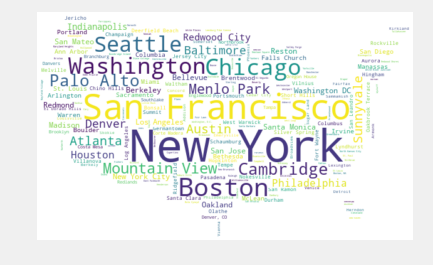
\includegraphics[width=.8\linewidth]{images/company_loc.png}
		\captionof{figure}{}
		\label{fig:test5}
	\end{minipage}%
	\begin{minipage}{.5\textwidth}
		\centering
		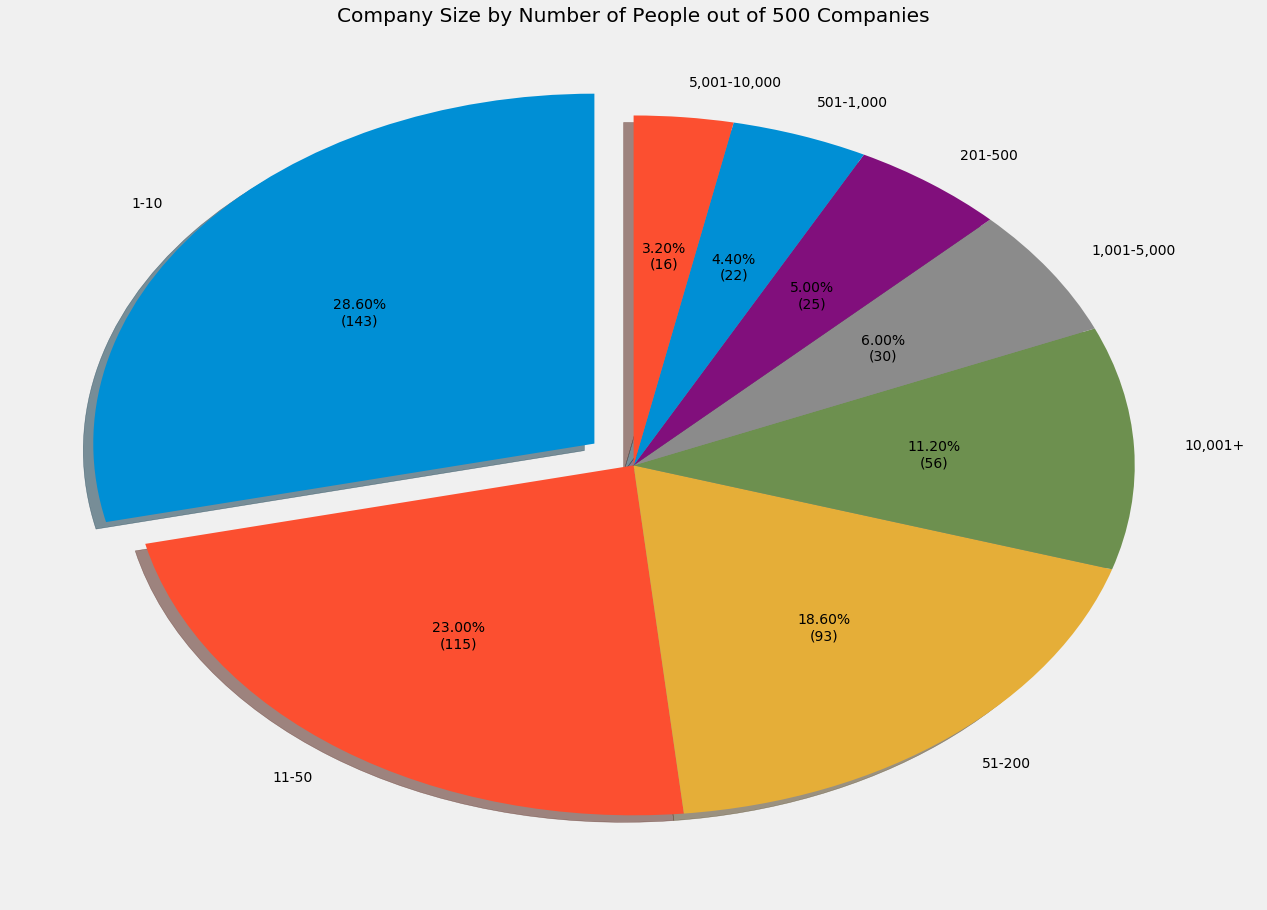
\includegraphics[width=.8\linewidth]{images/company_size.png}
		\captionof{figure}{}
		\label{fig:test6}
	\end{minipage}
\end{figure}

\subsection{Career Trajectory Prediction}
One aspect of our project was to be able to predict the type of company a person would work at given their schooling and first couple jobs.
To do this we decided to use our data from LinkedIn and Indeed to create tuples of users.
This data, as aforementioned, was scraped and converted into the following tuples: \emph{(School, Company1, Company2, Company3).}
Around 600 user tuples were generated from our web scraping.
The first step of preprocessing was to index the schools against the Times Higher Education, World University Rankings 2018 \cite{timesHigher}. Schools of rank 0-50 were bucketed as T1, 50-200 as T2, 200-500 as T3, 500-1000 as T4. Schools not on the list were given T5, and users without schooling were given T6 known as 'NONE'.
For companies the same process was performed, except the indexes were matched from Fortune 500, Top 1000 Companies \cite{fortune500}.
After this was completed the buckets were transformed back into integers (0 to 5) for use in various classifier softwares. Now having tuples of type (int, int, int, int) we could use many of \emph{sklearn}'s classifiers.
The classifiers would be trained on the tuples, considers \emph{School}, \emph{Company1}, and \emph{Company2} as the features and \emph{Company3} as the class.
For each classifier 550 tuples would be used for training and 85 would be used for testing. 
The first classifier used was a \emph{DecisionTree}, it resulted in a 66\% accuracy. The next classifier sued was an \emph{ExtraDecisionTree}, it resulted in a similar accuracy of around 66\%. Decision trees were chosen mainly because they are easy to visualize for this type of problem. The next classifier used was a \emph{MultinomialNB}, it resulted in 67\% accuracy. The final classifier used was a \emph{MLPClassifier}, it resulted in 68\% accuracy. From these results it's easy to see that the average accuracy was around 67\%. The testing was done using an 7 fold cross validation. An interesting finding from the visualization of the decision tree was that the only feature used to classify was \emph{Company2}. This leads us to believe that the most recent job you had is most likely to predict your next job, which falls in line with common sense.

\section{Conclusion}
In conclusion, our analysis provides a holistic view of the current education and job market. The creation of this project forced us to consider many of the aspects of \emph{knowledge discovery}. Choosing classifiers, proper preprocessing and finding apporpiate sources were among many of the important decisions we made. We also provide a unique approach to predicting career paths with self mined data using a tier based approach with various classification methods. Further, we executed text classification to predict industries aligned with certain job descriptions. Ultimately, our analysis yielded promising results which applied to more data could yield even more prominent results. 

\begin{acks}
	As an alternative to the .zip file uploaded on Blackboard, our code base is in a \href{https://github.com/jer96/CareerPathPrediction}{GitHub repository}.
The authors would like to thank Professor Jeibo Luo for a great semester and the oppurtunity to work on an interesting project.

\end{acks}

% Bibliography
\bibliographystyle{ACM-Reference-Format}
\bibliography{report-bibliography}
